\begin{frame}
\frametitle{Vulkan Instance}
\begin{columns}

\column{.6\textwidth}

\begin{itemize}
\item Dobbiamo creare un'istanza di Vulkan per accedere al resto dell'API
\item Quando creiamo un'istanza indichiamo i layer che vogliamo abilitare
\item I layer sono componenti opzionali che modificano il comportamento delle funzioni dell'API
\item Per esempio, possiamo usare un layer per controllare se il nostro utilizzo dell'API non violi la specifica
\item Quando creiamo un'istanza indichiamo le estensioni d'istanza che vogliamo abilitare
\item Le estensioni aggiungono nuove funzionalità all'API
\end{itemize}

\column{.4\textwidth}

\begin{figure}[ht]
    \centering
    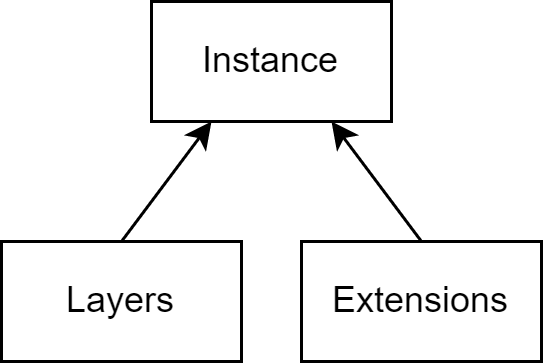
\includegraphics[scale=0.2]{images/SlidesInitializingVulkan/Instance.png}
\end{figure}

\end{columns}
\end{frame}
